\section{Computational Results}

We simulated performance of our algorithms on random graphs generated
by the graph models we outlined. In the following graphs each data
point is obtained by averaging the measurements over 10 random
graphs. Figures~\ref{fig:a=1:1} and \ref{fig:a=1:2} show that the
lower bound we calculated for the expected performance of the sampling
algorithm accurately captures the behavior of the sampling algorithm
when $a=1$. Indeed, the inequality we used is an accurate
approximation of the expectation, up to lower order terms. The random
sampling algorithm does well, both when $c$ is low and high, but
falters when $ck=1$. The greedy algorithm performs better than the
random sampling algorithm in all cases, but its advantage vanishes as
$c$ gets larger. Note that the dip in the graphs when $cl=ar$, at
$c=4$ in Figure~\ref{fig:a=1:1} and $c=2$ in Figure~\ref{fig:a=1:2} is
expected and was previously demonstrated in Figure 1.  In all the
plots below, the red, blue and yellow lines denote the approximation
ratio of the greedy, sampling and partitioning algorithms respectively
wrt the upper-bounds of the optimal that we described before.

\begin{figure}[h]
\centering
\begin{minipage}[h]{0.45\textwidth}
\centering
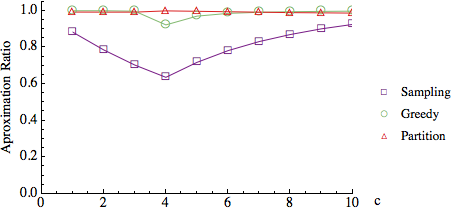
\includegraphics[width=0.8\textwidth]{images/l=25000,r=100000_Greedy_vs_Naive.png}
\caption{Approximation ratios when $|L|=25$k, $|R|=100$k, $d=20$, $a=1$}\label{fig:a=1:1}
\end{minipage}
\hspace{0.2cm}
\begin{minipage}[h]{0.45\textwidth}
\centering
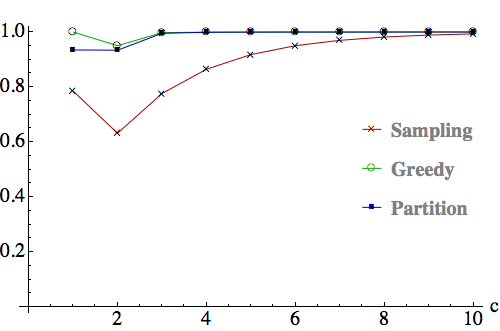
\includegraphics[width=0.8\textwidth]{images/l=50000,r=100000_Greedy_vs_Naive.png}
\caption{Approximation ratios when $|L|=50$k, $|R|=100$k, $d=20$, $a=1$}\label{fig:a=1:2}
\end{minipage}
\end{figure}


% Can we show the graph for larger c? Maybe up to 20?
% Also I can't believe that greedy is optimal. I am still tempted to say that
% greedy will do badly when d is small. Like d < 5.

In contrast to the case when $a=1$, the sampling algorithm performs
worse when $a>1$ but performs increasingly better with $c$ as
demonstrated by Figures~\ref{fig:a=2} and \ref{fig:a=4}. The greedy
algorithm continues to produce solutions that are nearly optimal,
regardless of the settings of $c$ and $a$. Therefore, our simulations
suggest that in many cases a software engineer can simply design the
sampling method for solving the $(c, a)$-recommendation subgraph
problem. In those cases where the sampling is not suitable we still
find that the greedy does adequately given its simplicity in
implementation.

\begin{figure}[h]
\centering
\begin{minipage}[h]{0.45\textwidth}
\centering
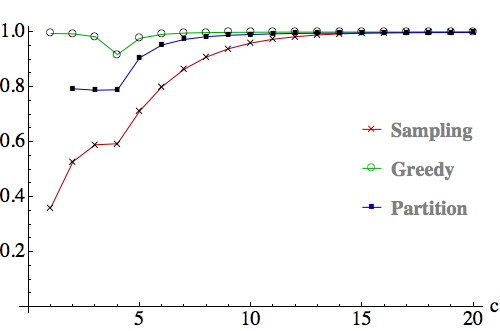
\includegraphics[width=0.8\textwidth]{images/l=50000,r=100000,a=2_Greedy_vs_Naive.png}
\caption{Approximation ratios when $|L|=50$k, $|R|=100$k, $d=20$, $a=2$}\label{fig:a=2}
\end{minipage}
\hspace{0.2cm}
\begin{minipage}[h]{0.45\textwidth}
\centering
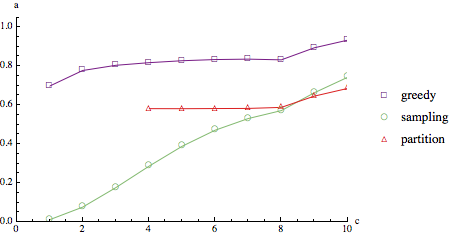
\includegraphics[width=0.8\textwidth]{images/l=50000,r=100000,a=4_Greedy_vs_Naive.png}
\caption{Approximation ratios when $|L|=50$k, $|R|=100$k, $d=20$, $a=4$}\label{fig:a=4}
\end{minipage}
\end{figure}
